% !TEX program = xelatex
\documentclass[11pt,a4paper]{article}

\usepackage[spanish]{babel}
\usepackage{graphicx}
\usepackage{geometry}
\usepackage{fancyhdr}
\usepackage{xcolor}
\usepackage{hyperref}
\usepackage{amsmath}
\usepackage{booktabs}
\usepackage{tabularx}
\usepackage{array}
\usepackage{longtable}
\usepackage{float}
\usepackage{caption}
\usepackage{subcaption}
\usepackage{enumitem}
\usepackage{tikz}
\usepackage{microtype}

\newcolumntype{L}{>{\raggedright\arraybackslash}X}
\newcolumntype{C}{>{\centering\arraybackslash}X}

\geometry{top=2.4cm,bottom=2.4cm,left=2.2cm,right=2.2cm,headheight=14pt}

\hypersetup{
  colorlinks=true,
  linkcolor=blue,
  urlcolor=blue,
  pdftitle={Memoria Fase III - SOM CUDA},
  pdfauthor={Grupo 1}
}

\pagestyle{fancy}
\fancyhf{}
\fancyhead[L]{Arquitectura de Computadores - Fase III}
\fancyhead[R]{Grupo 1}
\fancyfoot[R]{\thepage}

\setlist[itemize]{itemsep=0.25em,topsep=0.4em}
\setlist[enumerate]{itemsep=0.25em,topsep=0.4em}

\graphicspath{{assets/}{docs/memoria-fase3/assets/}}

\begin{document}

% ============================================================
% PORTADA
% ============================================================
\pagenumbering{gobble}
\begin{titlepage}
\thispagestyle{empty}
\begin{tikzpicture}[remember picture,overlay]
    \node at (current page.center) {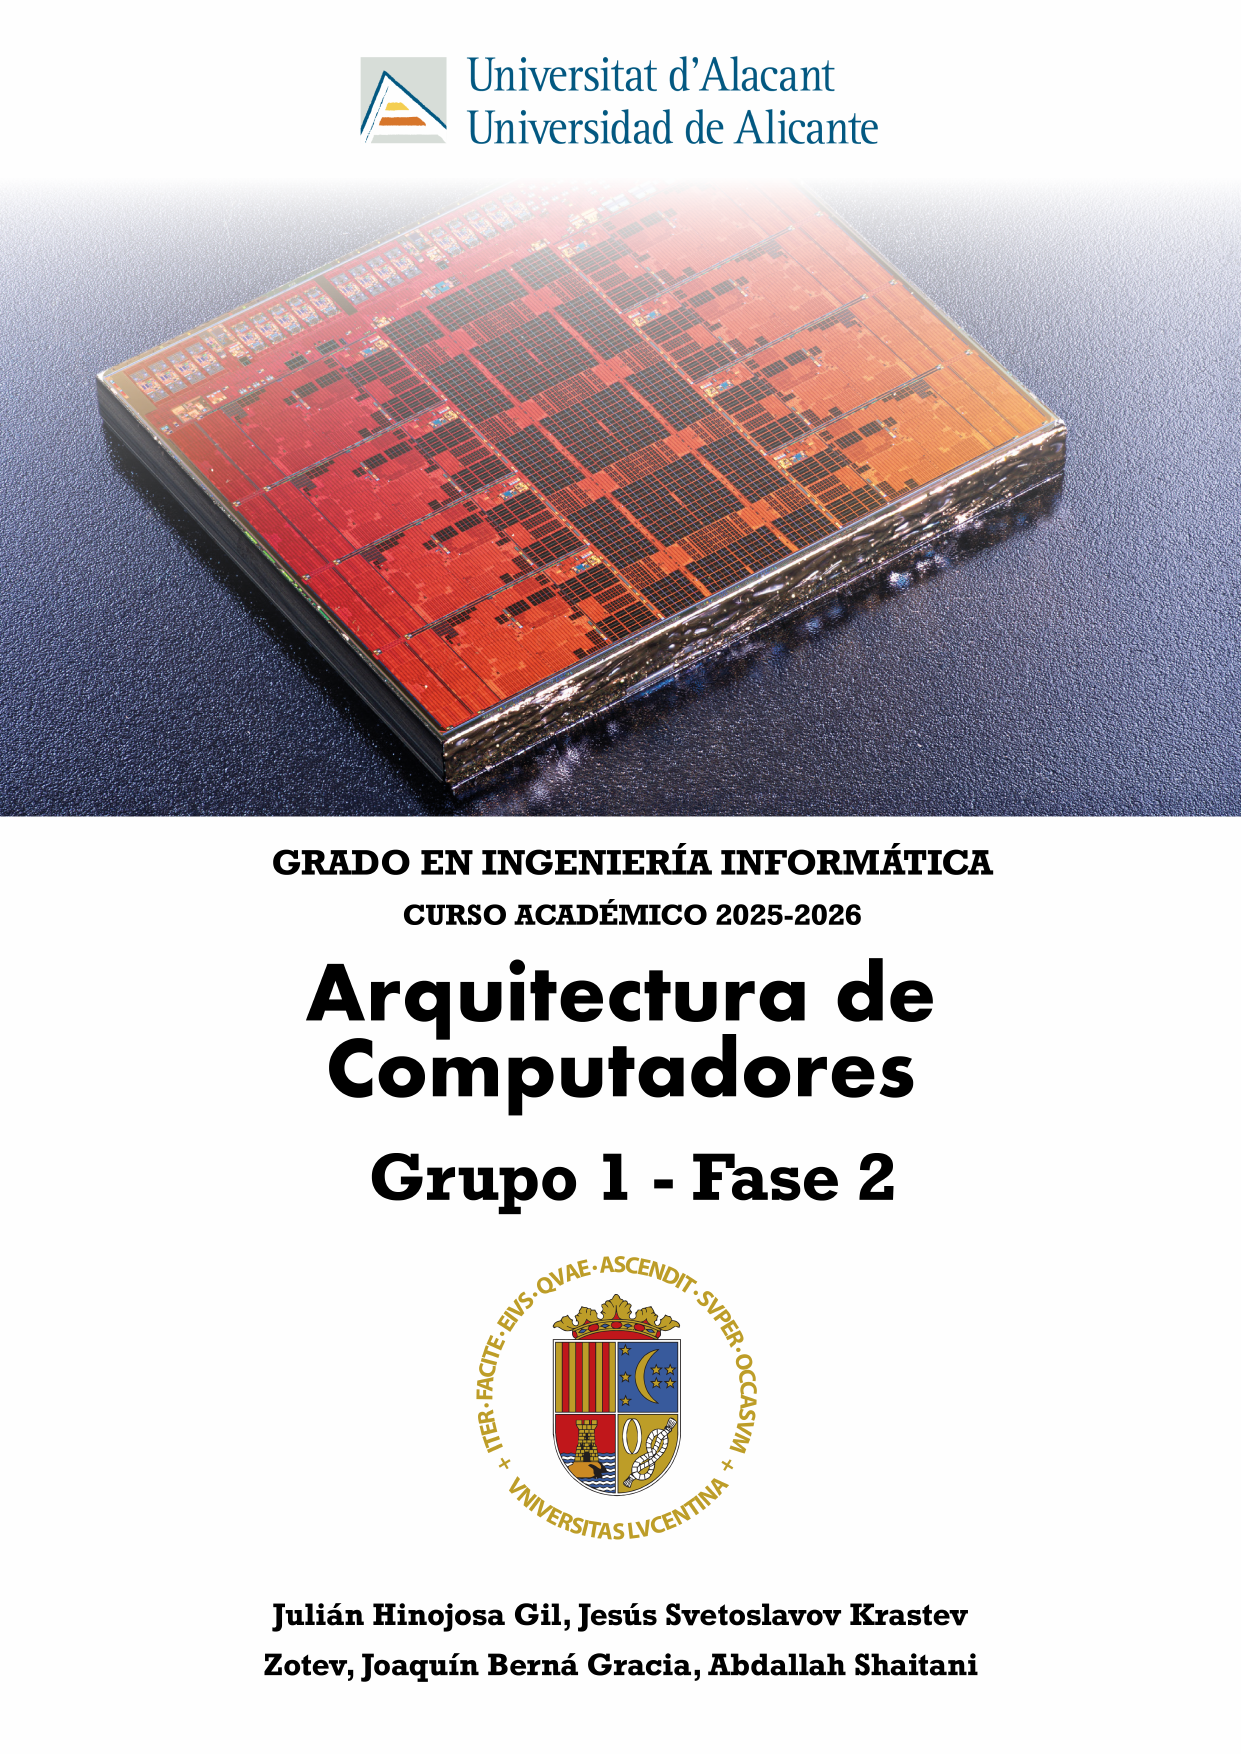
\includegraphics[width=\paperwidth,height=\paperheight]{portada_base.png}};
    % Cubrimos la zona inferior del texto original para reconstruir la capa textual en LaTeX.
    \fill[white] ([yshift=0cm]current page.south west) rectangle ([yshift=15.6cm]current page.south east);

    \node[align=center] at ([yshift=13.9cm]current page.south) {\fontsize{22}{26}\selectfont\bfseries Arquitectura de Computadores};
    \node[align=center] at ([yshift=12.5cm]current page.south) {\fontsize{16}{20}\selectfont\bfseries Grupo 1 -- Fase 3};
    \node[align=center] at ([yshift=11.4cm]current page.south) {\fontsize{14}{18}\selectfont Grado en Ingeniería Informática};
    \node[align=center] at ([yshift=10.6cm]current page.south) {\fontsize{13}{16}\selectfont Curso académico 2025--2026};

    \node[align=center] at ([yshift=8.9cm]current page.south) {\fontsize{13}{16}\selectfont\bfseries Memoria técnica de implementación y optimización};
    \node[align=center,text width=0.82\paperwidth] at ([yshift=7.2cm]current page.south) {\large
    Julián Hinojosa Gil \;\textbullet\; Jesús Svetoslavov Krastev Zotev \\
    Joaquín Berná Gracia \;\textbullet\; Abdallah Shaitani};

    \node[align=center] at ([yshift=2.1cm]current page.south) {\large Mayo de 2026};
\end{tikzpicture}
\mbox{}
\end{titlepage}

\newpage
\tableofcontents
\newpage

\pagenumbering{arabic}
\setcounter{page}{1}

% ============================================================
% CUERPO
% ============================================================
\section{Intro}

Esta memoria resume el trabajo realizado en la \textbf{Fase III grupal} de Arquitectura de Computadores sobre un clasificador basado en \textbf{Self-Organizing Maps (SOM)} acelerado con CUDA. El objetivo del proyecto no era solo obtener una versión funcional en GPU, sino construir una implementación que reprodujera exactamente el resultado de la CPU y que además mejorara su tiempo de ejecución en el entorno del laboratorio.

La idea general del problema es simple: para cada patrón de entrada hay que decidir qué neurona del mapa SOM lo representa mejor. La dificultad aparece al trasladar esa lógica a GPU, porque la estructura de datos original, el coste de las transferencias y la forma de localizar la neurona ganadora condicionan por completo el rendimiento.

\section{Problema y entorno de pruebas}

\subsection{Qué resuelve el programa}

El programa trabaja con un mapa SOM bidimensional formado por neuronas. Cada neurona almacena un vector de pesos y una etiqueta de clase. Para clasificar un patrón, se calcula su distancia euclídea respecto a cada neurona del mapa y, además, se añade la contribución del vecindario en cruz válido: arriba, abajo, izquierda y derecha. La neurona con la menor puntuación total determina la etiqueta de salida para ese patrón.

Dicho de forma más formal, si $p$ es un patrón, la distancia base de una neurona $(i,j)$ se obtiene comparando componente a componente el patrón con su vector de pesos. A partir de esa distancia base se construye una puntuación total que también tiene en cuenta el vecindario inmediato. La intuición es sencilla: no basta con que una neurona individual se parezca al patrón; también interesa cómo encaja respecto a la zona local del mapa.

\begin{equation}
  d_{ij}(p)=\sqrt{\sum_{k=0}^{dim-1}(p_k-w_{ij,k})^2},
  \qquad
  s_{ij}(p)=d_{ij}(p)+\sum_{(u,v)\in N_{ij}} d_{uv}(p)
\end{equation}

donde $N_{ij}$ representa los vecinos válidos de $(i,j)$ en forma de cruz. En los bordes y esquinas el número de vecinos disminuye, así que el kernel tiene que comprobar límites explícitamente antes de sumar contribuciones.

\begin{figure}[H]
\centering
\begin{tikzpicture}[scale=0.9]
  \foreach \x in {0,1,2} {
    \foreach \y in {0,1,2} {
      \draw[gray!60] (\x,\y) rectangle ++(1,1);
    }
  }
  \fill[blue!18] (1,1) rectangle ++(1,1);
  \fill[green!18] (1,2) rectangle ++(1,1);
  \fill[green!18] (1,0) rectangle ++(1,1);
  \fill[green!18] (0,1) rectangle ++(1,1);
  \fill[green!18] (2,1) rectangle ++(1,1);

  \node at (1.5,1.5) {\small Neu};
  \node at (1.5,2.5) {\small Arriba};
  \node at (1.5,0.5) {\small Abajo};
  \node at (0.5,1.5) {\small Izq.};
  \node at (2.5,1.5) {\small Dcha.};
\end{tikzpicture}
\caption{Vecindario en cruz usado por la clasificación}
\label{fig:vecindario-cruz}
\end{figure}

En la práctica intervienen tres bloques de datos:
\begin{itemize}
  \item \texttt{SOM}: estructura del mapa, con alto, ancho, dimensión y matriz de neuronas.
  \item \texttt{Patrones}: conjunto de vectores de entrada a clasificar.
  \item \texttt{EtiquetaCPU} y \texttt{EtiquetaGPU}: arrays con una etiqueta de salida por patrón.
\end{itemize}

La corrección se valida con \texttt{runTest}, que ejecuta tanto la versión secuencial como la versión CUDA y compara los resultados. La GPU solo se considera correcta si para todos los patrones se cumple la igualdad \texttt{EtiquetaGPU[i] == EtiquetaCPU[i]}. Solo a partir de esa condición tiene sentido interpretar el tiempo GPU y el factor de aceleración frente a CPU.

\subsection{Entorno y datasets usados}

Las pruebas se realizaron pensando en el entorno objetivo del aula:
\begin{itemize}
  \item compilación con \textbf{Visual Studio + CUDA};
  \item perfilado con \textbf{Nsight Compute};
  \item GPU objetivo tipo \textbf{GTX 1660 Super} (arquitectura Turing).
\end{itemize}

Durante la práctica se trabajó con dos datasets principales:
\begin{itemize}
  \item \textbf{Dataset pequeño}: SOM \texttt{32x32}, dimensión \texttt{64}. Se utilizó como entorno de validación rápida durante el desarrollo.
  \item \textbf{Dataset grande}: SOM \texttt{128x128}, dimensión \texttt{256}. Se utilizó como escenario principal de evaluación y es la base de las tablas y capturas que se muestran en esta memoria.
\end{itemize}

Los dos escenarios son útiles, pero no comparables entre sí de forma directa. El dataset pequeño sirve para comprobar rápidamente si una idea va en la dirección correcta, mientras que el grande deja ver con más claridad qué cambios mejoran de verdad el comportamiento del programa bajo carga. Para mantener la memoria uniforme, los resultados y capturas del bloque de optimizaciones se presentan sobre el dataset grande. Las capturas y reportes usados para sostenerlos se conservan en la carpeta \texttt{profiling/}.

\section{Implementación baseline}

\subsection{Qué hubo que construir primero}

La función GPU no podía limitarse a copiar la lógica de CPU tal cual, porque la representación original del programa estaba pensada para trabajar con punteros dinámicos, no con memoria lineal en device. Antes de hablar de optimización hubo que hacer un trabajo de base para que existiera una primera versión funcional en GPU.

Ese trabajo consistió en aplanar la información necesaria del mapa y de los patrones, preparar buffers contiguos y mover los datos a la GPU de una forma razonable. En otras palabras, la baseline no fue simplemente ``la versión sin optimizar'', sino la primera versión en la que el problema ya estaba adaptado a un formato que la GPU podía ejecutar sin romper la corrección.

Esa adaptación también obligó a separar mejor responsabilidades. En CPU era natural pensar en neuronas, punteros y estructuras enlazadas por conveniencia de programación; en GPU hacía falta pensar en bloques de memoria contigua, índices lineales y recorridos repetibles por miles de hilos. Buena parte del trabajo inicial consistió precisamente en traducir el problema desde una estructura ``cómoda de programar'' a una estructura ``razonable de ejecutar''.

\begin{table}[H]
\centering
\caption{Contrato básico de datos en la baseline GPU}
\label{tab:baseline-datos}
\begin{tabularx}{\textwidth}{>{\bfseries}l L}
\toprule
Buffer & Papel dentro de la clasificación \\
\midrule
\texttt{pesosSOM} & Copia lineal del mapa de pesos que permite recorrer la red completa desde GPU sin punteros dobles. \\
\texttt{patrones} & Bloque contiguo con todos los vectores de entrada a clasificar. \\
\texttt{distancias/puntuaciones} & Buffer intermedio donde M3 deja una puntuación por neurona antes de reducir. \\
\texttt{etiquetas} & Resultado final por patrón, una vez M4 localiza la mejor neurona. \\
\bottomrule
\end{tabularx}
\end{table}

\subsection{Flujo de la primera versión funcional}

Una vez construida esa base, el flujo general de clasificación quedó reducido a cuatro pasos:

\begin{table}[H]
\centering
\caption{Flujo conceptual de la versión baseline}
\label{tab:baseline-flujo}
\begin{tabularx}{\textwidth}{>{\bfseries}l L}
\toprule
Paso & Qué hace \\
\midrule
1 & Carga el mapa SOM y los patrones desde fichero. \\
2 & Prepara la información en buffers lineales y la envía a la GPU. \\
3 & Para cada patrón, calcula en GPU la puntuación de todas las neuronas y ejecuta una reducción para localizar la mejor. \\
4 & Escribe la etiqueta ganadora y, al final, compara GPU frente a CPU. \\
\bottomrule
\end{tabularx}
\end{table}

Desde esa primera versión ya existían las dos piezas esenciales del diseño final:
\begin{itemize}
  \item una fase tipo \texttt{M3}, encargada de calcular puntuaciones por neurona;
  \item una fase tipo \texttt{M4}, encargada de decidir la neurona ganadora mediante reducción.
\end{itemize}

La baseline cerró la corrección funcional y permitió medir la GPU frente a CPU, pero todavía estaba lejos de ser competitiva en tiempo. Aun así, esa primera construcción fue imprescindible, porque sin un contrato de datos estable y sin una separación clara entre cálculo masivo y reducción no habría sido posible iterar después con criterio.

\subsection{Por qué la baseline no era suficiente}

La baseline reveló cuatro problemas que marcaron toda la evolución posterior. El primero era estructural: trabajar en CPU con punteros dobles es cómodo, pero en GPU complica el acceso eficiente a memoria. El segundo era el coste de transferencia: si los datos se mueven con demasiada frecuencia, la GPU pasa demasiado tiempo esperando y demasiado poco calculando.

El tercero tenía que ver con el patrón de acceso a memoria global. Aunque los datos ya estuvieran linealizados, el orden en el que se recorrían los pesos seguía sin favorecer a los warps. El cuarto problema era la fase de reducción: encontrar la neurona con la menor puntuación seguía siendo una parte delicada, porque una reducción poco escalable hace que el resto del paralelismo se desaproveche.

En conjunto, la baseline funcionaba, pero todavía dedicaba demasiado esfuerzo a mover datos, accedía a memoria de forma mejorable y no exprimía la GPU en la fase final de selección.

\section{Optimizaciones}

La evolución del proyecto se puede leer en el orden real en el que se fueron consolidando los resultados. Ese orden coincide con los artefactos almacenados en \texttt{profiling/}: primero la baseline junto con \texttt{opt1} y \texttt{opt2}, y después la secuencia \texttt{opt3} a \texttt{opt8}. En esta memoria toda esa evolución se presenta ya sobre el dataset grande para que las comparaciones visuales y numéricas se hagan siempre dentro del mismo escenario.

\begin{table}[H]
\centering
\caption{Mapa rápido de la secuencia de optimizaciones}
\label{tab:ruta-opt}
\begin{tabularx}{\textwidth}{>{\bfseries}l L L}
\toprule
Versión & Idea principal & Efecto dominante buscado \\
\midrule
Opt1 & Reordenar pesos a SoA & Mejorar coalescencia y acceso a memoria global \\
Opt2 & Reducción en dos fases & Escalar mejor la búsqueda del mínimo \\
Opt3 & Warp shuffle & Afinar la reducción final dentro del warp \\
Opt4 & \texttt{--use\_fast\_math} & Reducir coste aritmético de operaciones frecuentes \\
Opt5 & Ajuste de grid en M4.2 & Aprovechar mejor el paralelismo de la fase final \\
Opt6 & Separar M3.1 / M3.2 con stencil & Evitar recomputación y reutilizar distancias \\
Opt7 & Loop unrolling & Recortar sobrecostes del bucle interno de distancia \\
Opt8 & Eliminar shared en M3.1 & Quitar un coste fijo que ya no compensaba \\
\bottomrule
\end{tabularx}
\end{table}

\subsection{Primera ronda de optimización}

La primera mejora relevante fue \textbf{SoA}, que corresponde a \texttt{opt1}. El problema era que, aun teniendo los datos linealizados, los pesos del SOM seguían almacenados en un layout que no ayudaba a la GPU. Pasar de un esquema por neurona a un esquema por componente permitió que hilos vecinos accedieran a posiciones más contiguas en memoria global. Esa idea no cambia el algoritmo, pero sí cambia cómo lo ve el hardware, y por eso el efecto en tiempo fue inmediato.

La segunda mejora de esta ronda fue la \textbf{reducción en dos fases}, que corresponde a \texttt{opt2}. Una vez acelerado el cálculo de puntuaciones, seguía haciendo falta mejorar la forma de encontrar el mínimo global. La solución fue dividir la reducción en una primera fase multibloque, donde se obtienen mínimos locales, y una segunda fase donde esos resultados se colapsan hasta el ganador final. De esta forma la reducción deja de depender de un único bloque y pasa a escalar mejor cuando el número de neuronas crece.

Visto desde fuera, esta primera ronda resolvió dos problemas distintos que estaban mezclados en la baseline. SoA atacó el problema de \emph{cómo se leen los datos}, mientras que la reducción en dos fases atacó el problema de \emph{cómo se decide el ganador}. Separar ambos planos fue importante, porque evitó atribuir a una sola técnica mejoras que en realidad venían de cuellos de botella diferentes.

El efecto de esta primera ronda se resume en la tabla siguiente:

\begin{table}[H]
\centering
\caption{Evolución de tiempos y aceleración en la primera ronda (dataset grande)}
\label{tab:tiempos-primera-grande}
\begin{tabular}{lccc}
\toprule
\textbf{Versión} & \textbf{GPU (s)} & \textbf{CPU (s)} & \textbf{Speedup} \\
\midrule
Baseline & 1.175254 & 9.010929 & 7.667217x \\
Opt1 (SoA) & 0.531398 & 9.015031 & 16.964738x \\
Opt2 (Map-Reduce 2 fases) & 0.537347 & 9.042473 & 16.827998x \\
\bottomrule
\end{tabular}
\end{table}

La lectura más importante de esta tabla es doble: la transición a SoA fue claramente el salto fuerte de la primera ronda, porque redujo el tiempo GPU desde \texttt{1.175254s} hasta \texttt{0.531398s}, es decir, aproximadamente un \textbf{54.78\%}. La reducción en dos fases mantuvo la dirección correcta desde el punto de vista algorítmico y dejó preparada una estructura más escalable, pero en esta captura concreta del dataset grande quedó ligeramente por detrás de Opt1 y cerró en \texttt{0.537347s}. Eso refuerza una idea importante: no toda mejora estructural produce una bajada inmediata en todas las mediciones, aunque siga siendo necesaria para sostener optimizaciones posteriores.

\begin{figure}[H]
\centering
\begin{subfigure}[t]{0.32\textwidth}
  \centering
  
\includegraphics[width=\textwidth]{baseline.PNG}
  \caption{Baseline}
\end{subfigure}
\hfill
\begin{subfigure}[t]{0.32\textwidth}
  \centering
  
\includegraphics[width=\textwidth]{opt1.PNG}
  \caption{Opt1}
\end{subfigure}
\hfill
\begin{subfigure}[t]{0.32\textwidth}
  \centering
  
\includegraphics[width=\textwidth]{opt2.PNG}
  \caption{Opt2}
\end{subfigure}
\caption{Capturas representativas de la primera ronda de optimización sobre el dataset grande}
\label{fig:baseline-opt2}
\end{figure}

\subsection{Segunda ronda de optimización}

La segunda ronda mantuvo el mismo dataset grande y sigue exactamente la secuencia \texttt{opt3} a \texttt{opt8}. A estas alturas ya se estaba trabajando de forma estable sobre el escenario exigente del problema, así que cualquier ineficiencia quedaba mucho más expuesta y cada cambio podía interpretarse directamente en términos de rendimiento final.

El primer paso fue \textbf{warp shuffle} (\texttt{opt3}), que afinó la reducción final sustituyendo parte del intercambio por memoria compartida por intercambio en registros. El resultado fue positivo, pero moderado: mejoró la fase final, aunque sin provocar todavía un salto fuerte.

Después llegó \texttt{opt4}, asociado a \textbf{\texttt{--use\_fast\_math}}. Era una hipótesis razonable: si la GPU podía usar versiones más agresivas de ciertas operaciones matemáticas, quizá el tiempo bajaría sin tocar el diseño del kernel. En la práctica, el impacto fue pequeño y no cambió la tendencia general de rendimiento.

El siguiente ajuste fue \texttt{opt5}, donde se probó un \textbf{grid más agresivo en M4.2}. La intención era explotar mejor el hardware en la fase final de reducción. El cambio afinó ligeramente el tiempo, pero siguió sin atacar el cuello principal.

El gran salto apareció en \texttt{opt6}, con el \textbf{patrón stencil y la separación M3.1/M3.2}. Hasta ese momento, la puntuación de cada neurona y la suma del vecindario seguían demasiado acopladas. Separar una fase base, que calcula la distancia de cada neurona al patrón, de una segunda fase que reutiliza esas distancias para sumar el vecindario en cruz eliminó recomputación y cambió de manera clara el coste real del trabajo.

Este punto merece subrayarse, porque explica por qué algunas optimizaciones pequeñas apenas se notaron y, en cambio, \texttt{opt6} cambió por completo la curva de tiempos. Mientras \texttt{opt3}, \texttt{opt4} y \texttt{opt5} afinaban una estructura todavía costosa, el stencil modificó directamente la cantidad de trabajo útil que se hacía por patrón. No era una cuestión de ``hacer lo mismo un poco más rápido'', sino de evitar repetir operaciones que la GPU estaba recalculando sin necesidad.

Con ese cambio ya consolidado, \texttt{opt7} aplicó \textbf{loop unrolling} al cálculo de distancias. No fue una revolución conceptual, pero sí un ajuste útil: una vez resueltos los cuellos grandes, esta clase de refinamiento ayudó a recortar tiempo adicional.

Por último, \texttt{opt8} retiró el uso de \textbf{memoria compartida en M3.1}. La idea aquí no era cambiar el algoritmo, sino comprobar si el coste de copiar el patrón a shared y sincronizar el bloque estaba compensando realmente. En esta carga no lo hacía, así que la versión final quedó más simple y, al mismo tiempo, mantuvo el rendimiento conseguido.

La evolución completa de esta segunda ronda fue la siguiente:

\begin{table}[H]
\centering
\caption{Evolución de tiempos y aceleración en la segunda ronda (dataset grande)}
\label{tab:tiempos-grande}
\begin{tabular}{lccc}
\toprule
\textbf{Versión} & \textbf{GPU (s)} & \textbf{CPU (s)} & \textbf{Speedup} \\
\midrule
Opt3 (Warp shuffle) & 0.530957 & 9.131940 & 17.199027x \\
Opt4 (\texttt{--use\_fast\_math}) & 0.531465 & 9.111363 & 17.143852x \\
Opt5 (Grid máx. M4.2) & 0.527902 & 9.092595 & 17.224012x \\
Opt6 (Patrón stencil) & 0.123489 & 10.162924 & 82.298547x \\
Opt7 (Loop unrolling) & 0.093351 & 9.045244 & 96.895403x \\
Opt8 (Sin shared M3.1, media 3 corridas) & 0.093599 & 9.093131 & 97.158663x \\
\bottomrule
\end{tabular}
\end{table}

Para la versión final Opt8 se realizaron tres corridas: GPU \texttt{0.094644s}, \texttt{0.092512s} y \texttt{0.093641s}, con speedups de \texttt{95.682380x}, \texttt{97.972216x} y \texttt{97.821392x}. Tomando la media oficial, la mejora global desde Opt3 fue de aproximadamente \textbf{82.37\%} menos tiempo GPU.

\begin{figure}[H]
\centering
\begin{subfigure}[t]{0.32\textwidth}
  \centering
  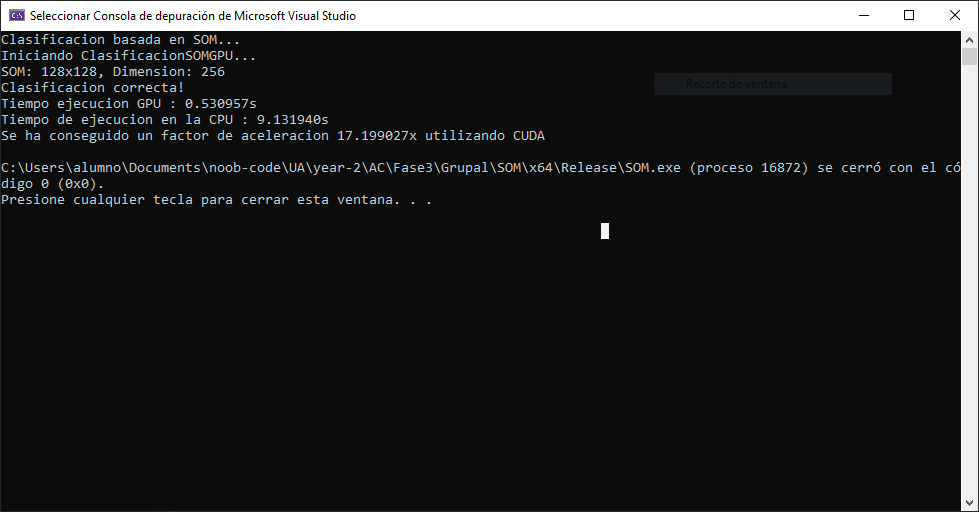
\includegraphics[width=\textwidth]{opt3.PNG}
  \caption{Opt3}
\end{subfigure}
\hfill
\begin{subfigure}[t]{0.32\textwidth}
  \centering
  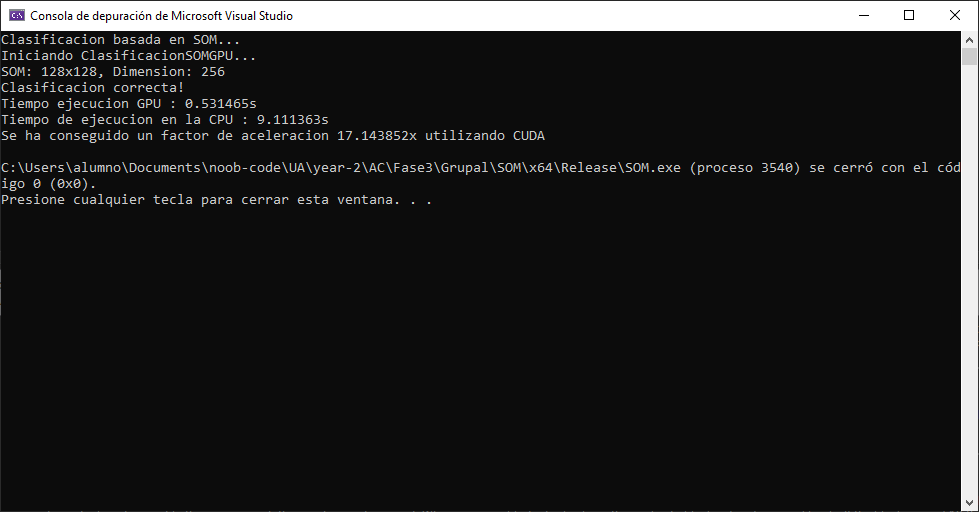
\includegraphics[width=\textwidth]{opt4.PNG}
  \caption{Opt4}
\end{subfigure}
\hfill
\begin{subfigure}[t]{0.32\textwidth}
  \centering
  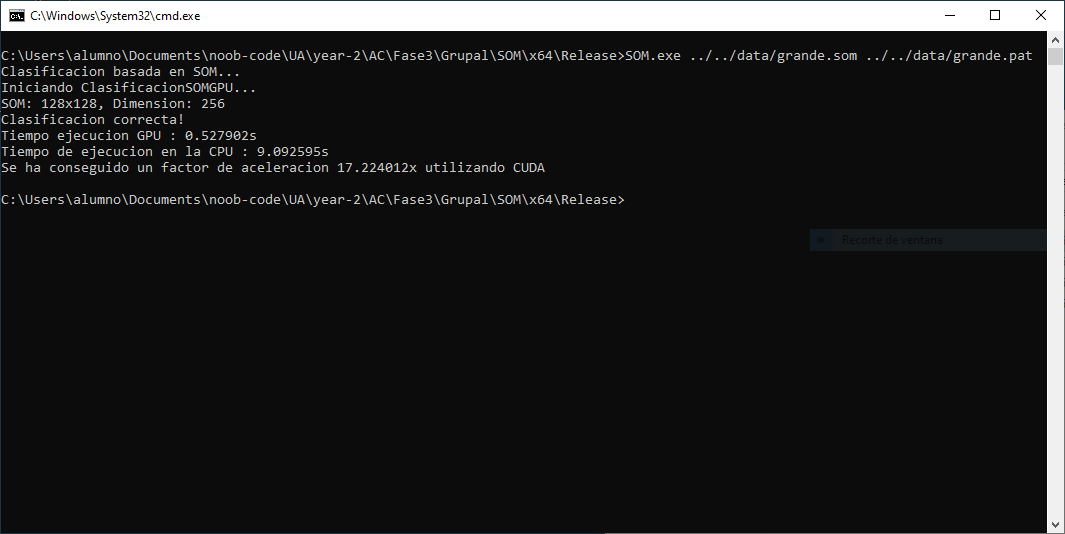
\includegraphics[width=\textwidth]{opt5.PNG}
  \caption{Opt5}
\end{subfigure}

\vspace{0.5em}

\begin{subfigure}[t]{0.32\textwidth}
  \centering
  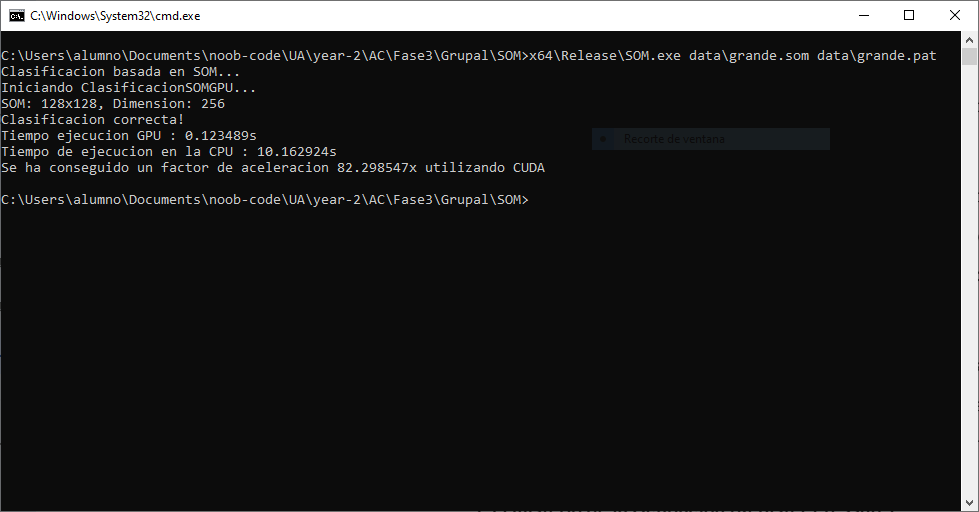
\includegraphics[width=\textwidth]{opt6.PNG}
  \caption{Opt6}
\end{subfigure}
\hfill
\begin{subfigure}[t]{0.32\textwidth}
  \centering
  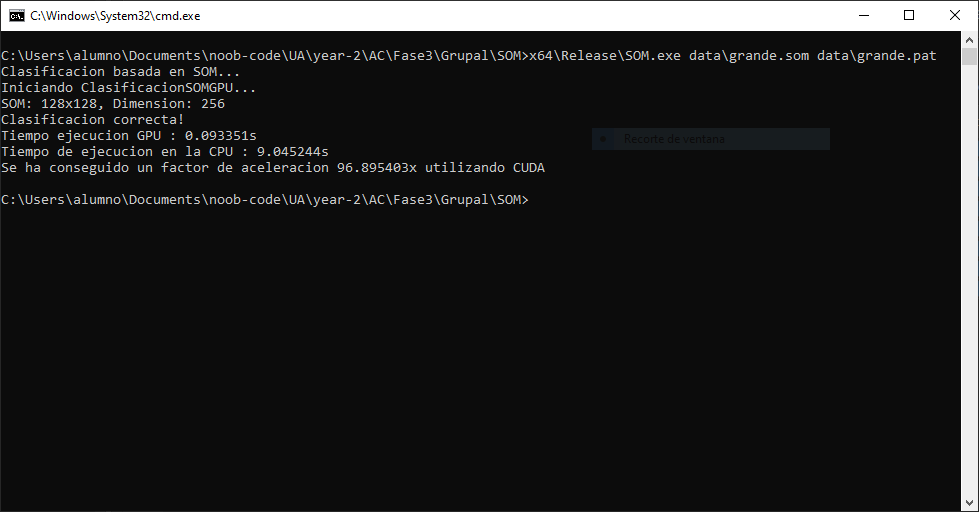
\includegraphics[width=\textwidth]{opt7.PNG}
  \caption{Opt7}
\end{subfigure}
\hfill
\begin{subfigure}[t]{0.32\textwidth}
  \centering
  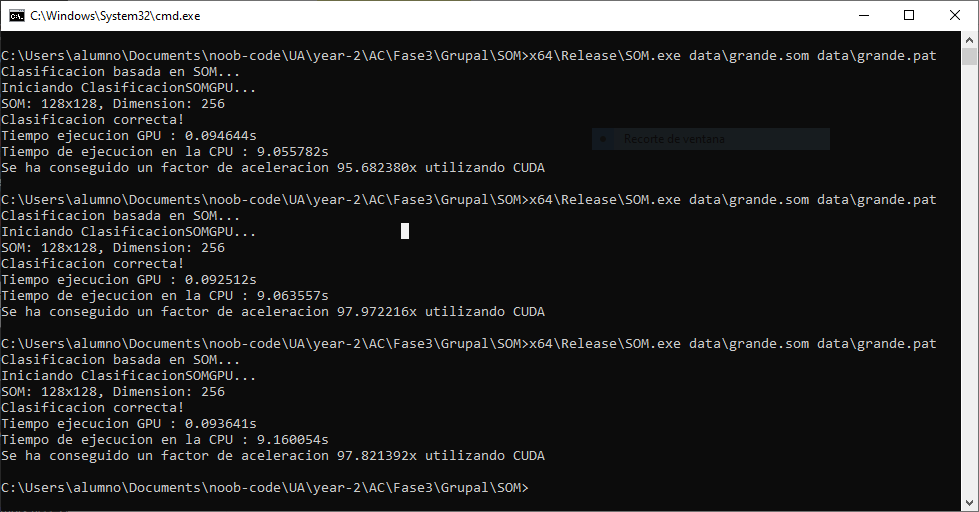
\includegraphics[width=\textwidth]{opt8.PNG}
  \caption{Opt8}
\end{subfigure}
\caption{Capturas representativas de la segunda ronda de optimización}
\label{fig:opt3a8}
\end{figure}

\subsection{Cambios y arreglos complementarios}

No todas las mejoras del proyecto consistieron en cambiar kernels para bajar unas décimas. También hubo arreglos y cambios de soporte que ayudaron a que el programa fuera más robusto y más fácil de mantener.

Por un lado, se introdujo \textbf{temporización multiplataforma} para poder trabajar tanto en Windows como fuera del aula sin depender de una única API del sistema. Eso permitió validar y comparar comportamientos sin romper la compatibilidad con Visual Studio.

Por otro lado, se incorporaron correcciones de \textbf{robustez interna}. Entre ellas destacan la liberación centralizada de \texttt{EtiquetaCPU} y \texttt{EtiquetaGPU} mediante \texttt{LiberarEtiquetasRobusto}, así como el ajuste de \texttt{SOM.Dimension} al crear el mapa. Estos cambios no aparecen en las tablas de rendimiento, pero sí evitan errores de limpieza, estados inconsistentes y fallos difíciles de rastrear.

También se hizo una \textbf{reestructuración del proyecto} para separar con claridad el control principal, la lógica CPU, la entrada/salida y el núcleo CUDA. A eso se sumó la actualización de \texttt{SOM.vcxproj} para reflejar la estructura final y la normalización de nombres en los artefactos de profiling. Todo ello redujo el coste de experimentar y dejó el trabajo mejor preparado para futuras iteraciones.

Aunque estos cambios no sean tan vistosos como una tabla de speedups, fueron importantes por una razón práctica: sin ellos el proceso de probar ideas, comparar ejecuciones y depurar errores habría sido mucho más lento y mucho menos fiable. En un proyecto de este tipo, la ingeniería de soporte no compite con la optimización; la hace viable.

\section{Conclusiones}

\subsection{Qué optimización aportó más}

Si se toma como referencia el dataset grande, en la primera ronda el cambio más claro fue la transición a \textbf{SoA}, porque mejoró de forma visible el acceso a memoria global. En la segunda ronda, la optimización más determinante fue \textbf{separar M3 en una fase base y otra stencil}, ya que eliminó recomputación y provocó el mayor salto de tiempo observado.

\subsection{Qué hipótesis tuvieron poco impacto}

No todas las ideas razonables acabaron siendo decisivas. En esta práctica, \texttt{--use\_fast\_math} y el ajuste de grid en M4.2 tuvieron un efecto pequeño. El warp shuffle mejoró la reducción final, pero su impacto quedó muy por debajo de las optimizaciones que atacaban directamente el patrón de acceso a memoria y la reutilización de trabajo.

\subsection{Qué nos dijo el profiling}

Los reportes de Nsight apuntaron siempre en la misma dirección: el problema era principalmente \textbf{memory-bound}. Las señales más repetidas fueron \texttt{Small Grid}, \texttt{Stall Long Scoreboard} y accesos globales no ideales. Eso explica por qué las mejoras más efectivas no fueron las que cambiaban unas pocas instrucciones, sino las que alteraban el layout de datos, la reducción o la cantidad de trabajo redundante.

\subsection{Qué queda por explorar}

Si se quisiera seguir afinando la solución sin salir de las reglas de la práctica, las líneas naturales serían:
\begin{itemize}
  \item barrer sistemáticamente \texttt{BLOCK\_DIM\_X/Y\_M3}, \texttt{BLOCK\_SIZE\_M4} y \texttt{GRID\_SIZE\_M4} en la GPU objetivo;
  \item estudiar con más detalle el coste de memoria compartida y registros en M3.1;
  \item comparar variantes finales de reducción según tamaño de mapa.
\end{itemize}

Como cierre, los dos mensajes más importantes de la memoria son estos: en la primera etapa sobre el dataset grande se pasó de baseline a Opt1 con una reducción del tiempo GPU de aproximadamente \textbf{54.78\%}, mientras que Opt2 confirmó una estructura de reducción más sólida aunque en esa medición concreta quedara ligeramente por detrás. Después, en la segunda etapa, se pasó de Opt3 a Opt8(media) con una reducción de aproximadamente \textbf{82.37\%}. La mejora real vino de entender cómo estaban interactuando memoria, reducción y reutilización del trabajo, no de acumular microajustes sin dirección.

\end{document}
